\section{Stabilität / Frequenzverhalten von OpAmps}

\subsection{UTF des rückgekoppelten Verstärkers}

\begin{minipage}[c]{0.53\columnwidth}
    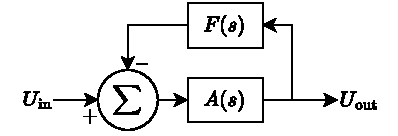
\includegraphics[width=\columnwidth, align=t]{images/10_stabilitaet_loop.pdf}
\end{minipage}
\hfill
\begin{minipage}[c]{0.46\columnwidth}
    \vspace{-0.2cm}
    \begin{align*}
         A_{\rm CL}(s)  &= \frac{U_{\rm out}(s)}{U_{\rm in}(s)} = \frac{A(s)}{1+ \underbrace{ A(s) F(s) }_{T(s)}} \\
                        &= \frac{1}{\frac{1}{A(s)} + F(s)} \overset{\text{tiefe Freq.}}{\approx} \frac{1}{F(s)}
    \end{align*}
\end{minipage}

\begin{ctabular}{ll | ll}
    $A(s)$  & Frequenzgang des Verstärkers      & $T(s)$    & Loop Gain     \\
    $F(s)$  & Frequenzgang der Rückkopplung     &           &               \\
\end{ctabular}


\subsection{Stabilitätskriterien}
Der \textbf{Nenner} von $A_{\rm CL}(s)$ darf \textbf{nicht null} sein, da das System sonst schwingt. \\
Um die Stabilität zu beurteilen werden Verstärkungs- und Phasenmarge betrachtet.

\smallskip
Damit ein System stabil ist, müssen die beiden folgenden Bedingungen für Verstärkungsmarge und Phasenmarge erfüllt sein:


\begin{minipage}[t]{0.48\columnwidth}
    \paragraph{Verstärkungsmarge}

    Bei $\Phi = \qty{180}{\degree}$ ablesen:

    \[
        \text{GM} = g_M = \abs{A(s) \cdot T(s)} \overset{!}{<} 1
    \]

    \smallskip

    \paragraph{Phasenmarge}

    Bei Verstärkung $1$ bzw  $\qty{0}{\decibel}$ ablesen:
    \[
        \text{PM} = \varphi_M = \qty{180}{\degree} - \Phi \overset{!}{>} \qty{0}{\degree}
    \]
\end{minipage}
\hfill
\begin{minipage}[t]{0.48\columnwidth}
    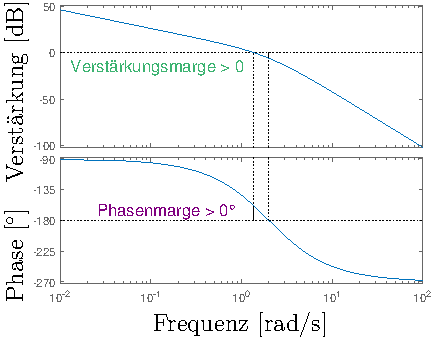
\includegraphics[width=\columnwidth, align=t]{images/10_bode_plot_V2.pdf}
\end{minipage}

% Für Stabilität muss die Verstärkungsmarge 
% \[
%     GM = g_M = \left.\abs{T(s)} \right|_{\angle T(S) = 180^\circ} < 1
% \]
% sein.

% Die Phasenmarge muss
% \[
%     PM = \phi_M = 180^\circ - \Phi =  \left. 180^\circ - \angle T(s) \right|_{\abs{T(s)} > 0^\circ}
% \]
% erfüllen.


\subsubsection{Überschwingen der Sprungantwort}

Die Phasenmarge bestimmt, wieviel die Sprungantwort überschwingt.

\vspace{-0.2cm}

\begin{ctabular}{ll}
    \textbf{Phasenmarge}                & \textbf{Verhalten der Sprungantwort}              \\
    $\phi_M \leq \qty{0}{\degree}$      & Gegengekoppelter Verstärker schwingt selbständig  \\
    $\phi_M > \qty{0}{\degree}$         & Stabil, mit gedämpftem Überschwingen              \\
    $\phi_M = \qty{65}{\degree}$        & Einziger Überschwinger mit $\qty{4.7}{\percent}$  \\
    $\phi_M \geq \qty{75}{\degree}$     & Einbussen bei der Slew-Rate                       \\
\end{ctabular}

\vspace{-0.2cm}



\subsection{OpAmp als System mit 2 Polen}

\begin{minipage}[c]{0.54\columnwidth}
    \begin{outline}
        \1 1. Pol (bei $f_{\rm d}$) bestimmt Bandbreite (GBW)
        \1 2. Pol (bei $f_{\rm nd}$) bestimmt die Stabilität \\
            \textrightarrow\ Phasenmarge $\varphi_M$
    \end{outline}
\end{minipage}
\hfill
\begin{minipage}[c]{0.42\columnwidth}
    \[
        \varphi_M = \qty{90}{\degree} - \arctan \left( \frac{\text{GBW}}{f_{\rm nd}} \right)
    \]
\end{minipage}


\subsubsection{Design-Regeln für Stabilität des OpAmps}

\begin{outline}
    \1 1. Pol muss in erster Stufe (Differenzstufe) realisiert werden
    \1 2. Pol bei ca. $3 \cdot \text{GBW}$ wählen \textrightarrow\ $\varphi_M \approx \qty{72}{\degree}$ (fast kein Überschwingen)
\end{outline}

